\documentclass[journal]{IEEEtran}

\usepackage{cite}
\usepackage{graphicx}
\usepackage{amsmath,amssymb,amsfonts}
\usepackage{booktabs}
\usepackage{array}
\usepackage[table]{xcolor}
\usepackage{url}
\usepackage[hidelinks]{hyperref}
\usepackage{placeins}
\usepackage{dblfloatfix}

\graphicspath{{figures/}}

\newcommand{\ie}{\textit{i.e.}}
\newcommand{\eg}{\textit{e.g.}}

\begin{document}

\title{A Pixel-to-Dimension Rule for Pooling Earth Embeddings}

\author{Isaac~Corley,
        Caleb~Robinson,
        Inbal~Becker-Reshef,
        and~Juan~M.~Lavista~Ferres
\thanks{Isaac Corley is with Taylor Geospatial, USA (e-mail: isaac.corley@taylorgeospatial.org).}
\thanks{Caleb Robinson, Inbal Becker-Reshef, and Juan M. Lavista Ferres are with Microsoft AI for Good Research Lab, USA.}
\thanks{Manuscript received XX, XX, 2026; revised XX, XX, 2026.}}

\markboth{IEEE Geoscience and Remote Sensing Letters}%
{Corley \MakeLowercase{\textit{et al.}}: A Pixel-to-Dimension Rule}

\maketitle

\begin{abstract}
Geospatial foundation models (GFMs) increasingly publish pixel-level embedding products that practitioners reuse without access to the encoder. Downstream patch- and region-level tasks must aggregate these dense embeddings into a single vector, yet pooling is usually treated as a default preprocessing step. We show that the ratio $N/D$ of pixels per region to embedding dimension predicts when higher-order pooling is reliable: fixed chips with $N \gg D$ benefit from distributional statistics, while variable-size parcels with $N \approx D$ expose covariance pooling as an unstable estimator. Across EuroSAT and PASTIS embeddings from AlphaEarth, OlmoEarth-Nano, and Tessera, distributional pooling reduces geographic generalization gaps on high-$N/D$ chips, but PASTIS acts as the failure case where covariance drops by more than 30\,pp and first-order summaries such as \emph{mean+std} and \emph{center-weighted} remain competitive. We give practitioners a one-step decision rule and release \emph{EuroSAT-Embed}, \emph{PASTIS-Embed}, and benchmark code.\footnote{Code: \url{https://github.com/isaaccorley/geopool}; data: \url{https://huggingface.co/datasets/isaaccorley/eurosat-embed} and \url{https://huggingface.co/datasets/isaaccorley/pastis-embed}.}
\end{abstract}

\begin{IEEEkeywords}
Geospatial foundation models, embeddings, pooling, land cover classification, crop classification, spatial generalization.
\end{IEEEkeywords}

\section{Introduction}
\IEEEPARstart{A}{} typical agricultural parcel in France covers 1.96\,ha---196 pixels at 10\,m resolution. A standard EuroSAT land-cover patch, by contrast, contains 4{,}096 pixels. Both settings require aggregating pixel embeddings from a geospatial foundation model (GFM) into a single patch-level vector, yet the number of pixels $N$ available for that summary differs by a factor of twenty. We show this difference, relative to the embedding dimension $D$, determines which pooling method wins.

\begin{figure}[t]
  \centering
  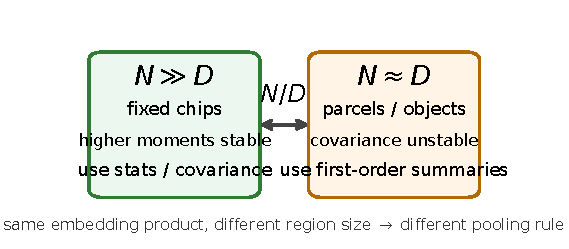
\includegraphics[width=\linewidth]{nd_rule.pdf}
  \caption{\textbf{A one-number rule for pooling.} When a labeled region has many more pixels than embedding dimensions ($N \gg D$), higher-order statistics can be estimated reliably and distributional pooling wins. When regions are small or variable-size ($N \approx D$ or $N < D$), covariance becomes ill-conditioned and first-order summaries are safer.}
  \label{fig:nd_rule}
\end{figure}

GFMs now publish dense pixel-level embeddings as downloadable data products~\cite{fang2026earthembeddingsproductstaxonomy,jakubik2023prithvi,cong2022satmae,bastani2023satlaspretrain,corley2025landsatbench}, enabling practitioners to reuse them without access to the underlying encoder. Many downstream tasks---crop mapping~\cite{kerner2025ftw,corley2025ftwprue,corley2025globalftw}, building detection, land-cover classification---assign a single label to a region rather than a pixel, requiring a post-hoc aggregation step. This \textit{input-label resolution mismatch}~\cite{workman2023handling} is ubiquitous: EuroSAT~\cite{helber2019eurosat} uses $64{\times}64$ patches, PASTIS~\cite{garnot2021panoptic} uses irregular agricultural parcels. The default aggregation---mean pooling---collapses each region to its average vector, discarding within-region variability that we show carries class signal.

Pooling is well-studied in image retrieval---generalized mean (GeM)~\cite{radenovic2018gem}, VLAD~\cite{jegou2010vlad}, NetVLAD~\cite{arandjelovic2016netvlad}, Fisher Vectors~\cite{perronnin2010improving}---and in temporal audio modeling~\cite{miech2017learnable}, but remains largely unexplored for GFM embeddings over irregular-polygon regions. The key challenge specific to this setting is that $N$ varies by three orders of magnitude across region types and sizes. When $N < D$, the sample covariance matrix has fewer data points than parameters and is mathematically rank-deficient; even at $N \approx D$ its eigenvalues are unstable, so second-order statistics estimated from such regions are unreliable. When $N \gg D$, those same statistics are well-conditioned and outperform mean pooling by a large margin. No prior work characterizes this transition or gives practitioners a decision rule.

We study post-hoc pooling across the full $N/D$ spectrum. Using pixel embeddings from three GFMs on two benchmarks, we benchmark 11 training-free and 2 fitted pooling operators and measure how method rankings shift with region size. Our contributions:
\begin{itemize}
  \item A practitioner-facing decision rule (Table~\ref{tab:cheatsheet}, Sec.~\ref{sec:results}): the ratio $N/D$ predicts when second-order operators (covariance, multi-moment stats) are viable, explaining the collapse of covariance pooling between EuroSAT ($N/D{=}64$) and small PASTIS parcels ($N/D{\lesssim}1$).
  \item A benchmark of 11 training-free and 2 fitted operators on EuroSAT (3 GFMs, random and spatial splits, kNN and linear probes) and PASTIS, showing distributional statistics shrink the EuroSAT random$\to$spatial accuracy gap from 9.6\,pp to 3.4\,pp on average (per-encoder reductions 43--76\%) (Sec.~\ref{sec:results}, Tables~\ref{tab:eurosat}--\ref{tab:pastis}).
  \item \emph{EuroSAT-Embed} and \emph{PASTIS-Embed}: pre-computed pixel-level embeddings from three GFMs, released with all benchmark code, providing the first controlled study of post-hoc pooling for GFM embedding products (Sec.~\ref{sec:data}).
\end{itemize}

\section{Data and Embeddings}
\label{sec:data}

\textbf{EuroSAT.} We use the 10-class EuroSAT land-cover dataset~\cite{helber2019eurosat}, which contains 27{,}000 Sentinel-2 patches at $64{\times}64$ pixels. We evaluate on both the standard random split~\cite{neumann2019domain} and a spatial split~\cite{ekim2025distribution,roberts2017cross} that partitions samples by longitude to reduce train-test leakage via spatial autocorrelation.

\textbf{PASTIS.} We use the PASTIS panoptic segmentation dataset~\cite{garnot2021panoptic}, which contains 2{,}433 Sentinel-2 time-series patches covering France with instance-level annotations of ${\sim}85{,}000$ agricultural parcels across 18 crop classes. Parcels are irregular polygons extracted from instance masks; parcel size varies from 5 to 3{,}440 pixels (median 196). We follow the official PASTIS train/test split using the folds released with the original paper (folds 1--4 train, fold 5 test). Parcels with fewer than 5 pixels are excluded.

\textbf{EuroSAT-Embed.} We construct pixel-level embedding datasets from AlphaEarth~\cite{brown2025alphaearth} (AEF, 64-d int8), OlmoEarth-Nano~\cite{herzog2025olmoearth} (128-d float32, $T{=}12$ subsampled time steps), and Tessera~\cite{feng2025tesseratemporalembeddingssurface} (128-d float32). All three products ultimately provide one embedding vector per output pixel. AEF and OlmoEarth take a time series of image patches and return a patch of pixel-aligned embeddings, so each output vector can reflect neighboring-pixel context; Tessera takes a time series for each pixel and returns a per-pixel embedding without adjacent-pixel context. We apply the same three encoders to PASTIS parcels to produce \emph{PASTIS-Embed}. We study pooling behavior, not encoder comparison.

\section{Pooling Methods}

We benchmark training-free operators that compress an $H{\times}W{\times}D$ embedding tensor ($N{=}HW$ pixels) into a single feature vector, plus two operators that fit a light additional stage on the training split.

\textbf{First-order statistics} ($D$-d): \textit{mean}, \textit{max}, generalized mean (\textit{GeM})~\cite{radenovic2018gem}, and \textit{center-weighted mean} (down-weighting boundary pixels).

\textbf{Distributional statistics} ($2D$--$5D$-d): \textit{std}, \textit{mean+std}, \textit{mean+max}, \textit{stats} (min/max/mean/std, $4D$-d), \textit{percentiles} ($5D$-d), \textit{median+IQR}, and \textit{covariance}~\cite{lin2015bilinear} (upper triangle, $D(D{+}1)/2$-d).

\textbf{Parametric (fit on train split)}: \textit{PCA} (mean-pooled then projected) and \textit{Bag of Visual Words} (\textit{BoVW})~\cite{csurka2004visual} (mini-batch $k$-means histogram).

In total we evaluate 11 training-free and 2 fitted operators.

\section{Experimental Setup}
We evaluate two probes: kNN ($k{=}5$, cosine distance) and multinomial logistic regression with regularization $C$ selected by 3-fold CV on the training split. We standardize before linear probing~\cite{corley2024revisiting}. Both probes are deterministic under our protocol; rerunning the linear probe with three seeds (0, 1, 42) yields identical accuracy ($\sigma{=}0$\,pp). EuroSAT results appear in Table~\ref{tab:eurosat} under random and spatial splits; PASTIS results (F1-macro) appear in Table~\ref{tab:pastis} (OE\,=\,OlmoEarth-Nano, Tess\,=\,Tessera).

\begin{table*}[!tb]
  \centering
  \setlength{\tabcolsep}{3pt}
  \footnotesize
  \caption{EuroSAT results (accuracy, \%): linear and kNN ($k{=}5$) probes under random and spatial splits. Best per column appears in \textbf{bold}; second-best is italicized. Dim\,=\,output embedding size relative to encoder dimension $D$. \colorbox{green!10}{\strut Stats} highlighted as the recommended method in the $N{\gg}D$ regime. $^*$OlmoEarth-Nano; OE\,=\,OlmoEarth; Tess\,=\,Tessera.}\label{tab:eurosat}
  \begin{tabular}{lc|cccc|cccc|cccc|cccc}
    \toprule
    & & \multicolumn{8}{c|}{Linear probe} & \multicolumn{8}{c}{kNN probe} \\
    \cmidrule(lr){3-10} \cmidrule(lr){11-18}
    & & \multicolumn{4}{c|}{Spatial split} & \multicolumn{4}{c|}{Random split} & \multicolumn{4}{c|}{Spatial split} & \multicolumn{4}{c}{Random split} \\
    \cmidrule(lr){3-6} \cmidrule(lr){7-10} \cmidrule(lr){11-14} \cmidrule(lr){15-18}
    Pooling & Dim & AEF & OE$^*$ & Tess & Avg & AEF & OE$^*$ & Tess & Avg & AEF & OE$^*$ & Tess & Avg & AEF & OE$^*$ & Tess & Avg \\
    \midrule
    Mean            & $D$              & 81.1 & 91.8 & 86.0 & 86.3 & 95.3 & 96.4 & 96.1 & 95.9 & 85.5 & 87.8 & 84.7 & 86.0 & 94.6 & 94.8 & 94.9 & 94.8 \\
    Std             & $D$              & 77.1 & 90.5 & 85.4 & 84.3 & 90.9 & 94.8 & 95.3 & 93.7 & 78.1 & 81.7 & 84.0 & 81.3 & 93.7 & 93.3 & 94.1 & 93.7 \\
    GeM             & $D$              & 83.2 & 91.7 & 87.3 & 87.4 & 95.5 & 95.9 & 96.4 & 95.9 & 85.7 & 86.6 & 85.4 & 85.9 & 94.6 & 93.3 & 95.1 & 94.3 \\
    Center-Weighted & $D$              & 85.7 & 91.9 & 87.6 & 88.4 & 96.1 & 96.8 & 96.1 & 96.3 & 86.0 & 87.8 & 85.5 & 86.4 & \textbf{95.4} & \textbf{95.0} & 95.5 & \textbf{95.3} \\
    Max             & $D$              & 86.1 & 90.6 & 89.8 & 88.8 & 92.9 & 92.9 & 93.7 & 93.2 & 80.5 & 85.5 & 80.8 & 82.3 & 90.5 & 91.4 & 92.5 & 91.5 \\
    \addlinespace[3pt]
    Mean+Std        & $2D$             & 84.2 & 93.4 & \textit{94.8} & 90.8 & \textit{96.1} & 96.6 & 97.1 & 96.6 & 86.4 & \textit{88.3} & 86.7 & \textit{87.1} & 94.9 & \textit{94.9} & 95.3 & \textit{95.0} \\
    Mean+Max        & $2D$             & \textit{89.1} & 93.3 & 94.4 & \textit{92.3} & 96.1 & 96.3 & 96.5 & 96.3 & 85.3 & 87.9 & 86.9 & 86.7 & 94.7 & 94.4 & \textbf{95.8} & 94.9 \\
    Median+IQR      & $2D$             & 81.7 & 93.2 & 88.4 & 87.7 & 94.8 & 95.9 & 95.9 & 95.5 & 86.0 & 86.0 & 85.7 & 85.9 & 94.1 & 94.0 & 94.4 & 94.1 \\
    Percentiles     & $5D$             & 85.6 & \textit{93.8} & 91.2 & 90.2 & 95.9 & \textit{97.0} & 97.0 & 96.6 & \textit{86.7} & 87.5 & 86.2 & 86.8 & 94.6 & 94.9 & 95.4 & 95.0 \\
    \rowcolor{green!10}
    Stats           & $4D$             & \textbf{91.0} & \textbf{94.0} & \textbf{94.9} & \textbf{93.3} & \textbf{96.2} & 96.6 & \textit{97.3} & \textit{96.7} & \textbf{86.9} & 87.6 & \textit{89.3} & \textbf{87.9} & \textit{95.0} & 94.4 & \textit{95.6} & 95.0 \\
    Covariance      & $D(D{+}1)/2$     & 89.1 & 93.4 & 93.7 & 92.1 & 95.8 & \textbf{97.2} & \textbf{97.6} & \textbf{96.8} & 84.4 & 84.8 & \textbf{89.8} & 86.4 & 93.4 & 94.3 & 94.5 & 94.1 \\
    \midrule
    \multicolumn{18}{l}{\textit{Parametric (fit on train split)}} \\[2pt]
    PCA             & $64$             & 79.7 & 91.6 & 80.8 & 84.0 & 95.2 & 95.6 & 95.0 & 95.3 & 85.3 & \textbf{88.4} & 86.1 & 86.6 & 93.5 & 94.1 & 92.7 & 93.5 \\
    BoVW            & $128$            & 88.9 & 88.2 & 88.7 & 88.6 & 94.4 & 94.5 & 96.3 & 95.1 & 84.0 & 82.1 & 87.4 & 84.5 & 90.7 & 90.3 & 90.2 & 90.4 \\
    \bottomrule
  \end{tabular}
\end{table*}

\begin{table}[!htbp]
  \centering
  \setlength{\tabcolsep}{2.5pt}
  \footnotesize
  \caption{PASTIS results (F1-macro, \%): linear and kNN ($k{=}5$) probes per encoder. Best per column appears in \textbf{bold}; second-best is italicized. \colorbox{blue!10}{\strut Mean+Std} highlighted as the recommended method for variable-size regions. OE\,=\,OlmoEarth-Nano; Tess\,=\,Tessera.}\label{tab:pastis}
  \begin{tabular}{l|cccc|cccc}
    \toprule
    & \multicolumn{4}{c|}{Linear probe} & \multicolumn{4}{c}{kNN probe} \\
    \cmidrule(lr){2-5} \cmidrule(lr){6-9}
    Pooling & AEF & OE & Tess & Avg & AEF & OE & Tess & Avg \\
    \midrule
    Mean            & 64.5 & 54.7 & \textit{49.0} & 56.1 & 56.5 & \textbf{41.1} & \textbf{43.8} & \textbf{47.1} \\
    Std             & 49.0 & 22.8 & 40.3 & 37.4 & 48.2 & 14.4 & 37.2 & 33.3 \\
    GeM             & 62.8 & 49.7 & 48.1 & 53.5 & 54.2 & 36.6 & 43.3 & 44.7 \\
    Center-Weighted & \textit{65.3} & \textit{54.8} & 48.9 & \textit{56.3} & \textbf{57.1} & \textit{40.3} & \textit{43.7} & \textit{47.0} \\
    Max             & 57.4 & 38.8 & 45.5 & 47.2 & 46.0 & 27.6 & 39.3 & 37.6 \\
    \addlinespace[2pt]
    \rowcolor{blue!10}
    Mean+Std        & \textbf{65.5} & \textbf{54.9} & 48.7 & \textbf{56.4} & \textit{56.7} & 39.7 & 43.5 & 46.6 \\
    Mean+Max        & 65.0 & 54.4 & 48.8 & 56.1 & 53.0 & 35.2 & 42.7 & 43.6 \\
    Median+IQR      & 64.3 & 50.8 & 48.4 & 54.5 & 55.7 & 35.7 & 43.3 & 44.9 \\
    Percentiles     & 65.3 & 52.4 & \textbf{49.4} & 55.7 & 56.6 & 39.1 & 43.0 & 46.3 \\
    Stats           & 65.0 & 54.0 & 48.4 & 55.8 & 52.1 & 34.3 & 42.5 & 43.0 \\
    Covariance      & 58.7 & 42.4 & 47.0 & 49.4 & 47.6 & 22.4 & 39.6 & 36.6 \\
    \midrule
    \multicolumn{9}{l}{\textit{Parametric (fit on train split)}} \\[1pt]
    PCA             & 64.4 & 47.9 & 48.2 & 53.5 & 56.2 & 38.8 & 43.3 & 46.1 \\
    BoVW            & 44.7 & 23.0 & 15.5 & 27.8 & 43.6 & 22.1 & 14.1 & 26.6 \\
    \bottomrule
  \end{tabular}
\end{table}


\section{Results}
\label{sec:results}

\textbf{The N/D ratio governs second-order viability.} The ratio of pixels per region $N$ to embedding dimension $D$ is a proxy for the conditioning of the sample second-moment estimator: the sample covariance is mathematically rank-deficient when $N < D$ and has unstable eigenvalues until $N$ is several times $D$. This directly explains the collapse of covariance pooling between EuroSAT and small PASTIS parcels; the ranking of first-order operators (mean variants) shifts more smoothly with region size and is not predicted by $N/D$ alone. EuroSAT patches have $N{=}4{,}096$ and $D{\in}\{64,128\}$, giving $N/D \geq 32$: second-order statistics are well-conditioned. PASTIS parcels have a median $N{=}196$; for OlmoEarth and Tessera ($D{=}128$) the median sits at $N/D{\approx}1.5$, and the smallest parcels in the dataset fall below $N{=}D$ entirely. Fig.~\ref{fig:nd_transition} visualizes the transition; this single structural quantity explains every major finding below.

\textbf{When $N \gg D$: distributional statistics win.} On EuroSAT spatial splits, \textit{stats} pooling reaches 91--95\% accuracy (avg.\ 93.3\%) vs.\ 81--92\% for \textit{mean} (avg.\ 86.3\%), a +7.0\,pp gain (Table~\ref{tab:eurosat}). \textit{Covariance} leads on random splits for two of three encoders (OlmoEarth: 97.2\%, Tessera: 97.6\%). Fig.~\ref{fig:gap_chart} shows that distributional methods are simultaneously more accurate and more robust: averaged across encoders, \textit{mean} drops 9.6\,pp from random to spatial splits while \textit{stats} drops only 3.4\,pp---a 65\% reduction (per-encoder: AEF 63\%, OlmoEarth 43\%, Tessera 76\%). \textit{Mean+max} (4.0\,pp) and \textit{covariance} (4.8\,pp) also exhibit small gaps. kNN trends are consistent, with \textit{stats} leading on spatial splits (avg.\ 87.9\%) and \textit{center-weighted mean} on random splits (avg.\ 95.3\%).

\begin{figure}[!ht]
  \centering
  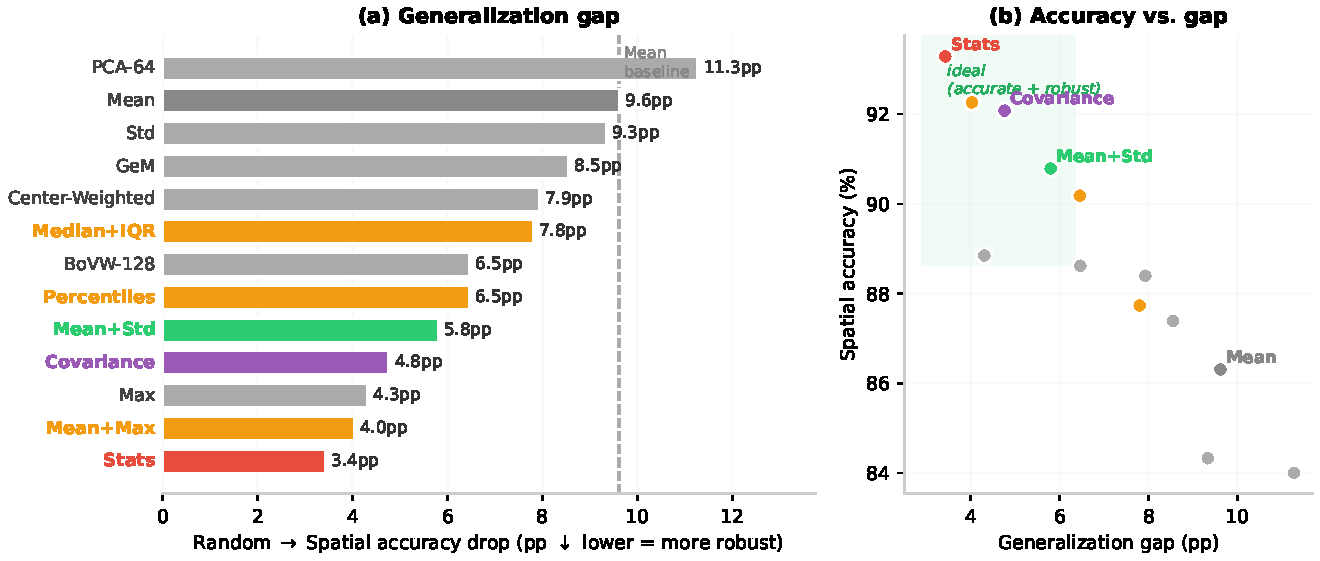
\includegraphics[width=\linewidth]{gap_chart.pdf}
  \caption{\textbf{Distributional pooling is more accurate and more robust under spatial shift.} (a) Accuracy drop when moving from a random to a geographically disjoint split, averaged across three GFMs---shorter bars are better. Mean pooling drops 9.6\,pp; stats drops only 3.4\,pp, a 65\% reduction. (b) Spatial accuracy vs.\ generalization gap per method. Methods in the upper-left are both accurate and robust; distributional methods cluster there while mean pooling sits lower-right.}
  \label{fig:gap_chart}
\end{figure}

\textbf{When $N \approx D$: PASTIS exposes the failure case.} EuroSAT makes covariance pooling look attractive because every labeled patch supplies thousands of pixels. PASTIS tests the opposite regime: labels are irregular parcels, many parcels have $N < D$, and the sample covariance matrix becomes rank-deficient. In this setting, \textit{covariance} falls from 89.1\% spatial accuracy on EuroSAT-AEF to 58.7\% F1 on PASTIS-AEF, and \textit{stats} similarly loses its EuroSAT advantage (Table~\ref{tab:pastis}). The practical lesson is not that PASTIS produces a large new accuracy win; rather, it shows where EuroSAT-derived pooling advice breaks. First-order summaries such as \textit{mean+std} (linear avg.\ 56.4\%), \textit{center-weighted mean} (56.3\%), and \textit{mean} (56.1\%) are numerically close and remain competitive because they preserve coarse distributional structure without requiring stable second moments. For kNN, \textit{mean} and \textit{center-weighted mean} are the strongest PASTIS choices, so our variable-region recommendation should be read as a conservative first-order family rather than a single universally dominant operator.

\begin{figure*}[t]
  \centering
  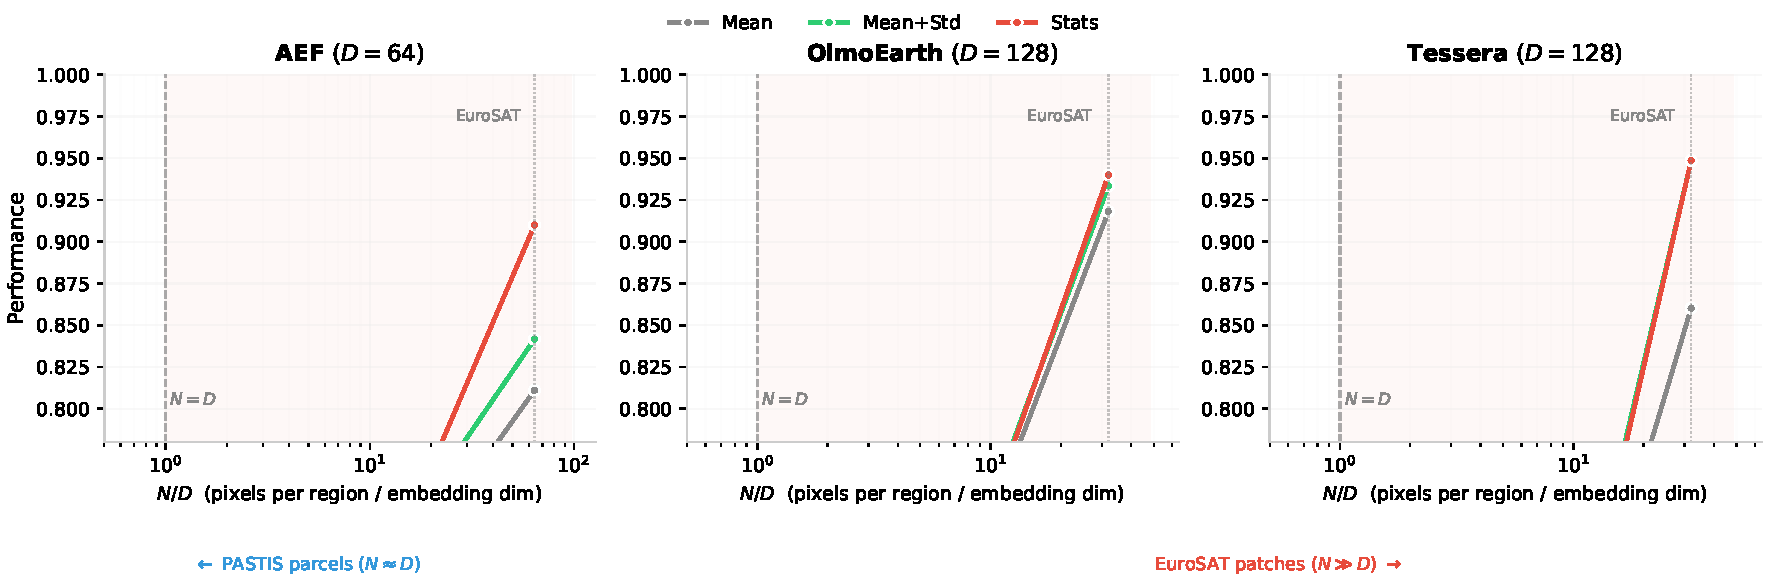
\includegraphics[width=\linewidth]{nd_phase_transition.pdf}
  \caption{\textbf{Pooling performance as a function of $N/D$, the ratio of pixels per region to embedding dimension.} Each panel shows per-bin F1 (PASTIS, four parcel-size bins) and accuracy (EuroSAT) plotted against $N/D$ on a log scale for one GFM. The dashed vertical line marks $N{=}D$. To the left, where parcels are small and $N \approx D$, covariance (purple) collapses because its sample estimate becomes rank-deficient, while mean+std remains strong. Moving right toward EuroSAT patches where $N \gg D$, covariance recovers and leads. Mean+std stays competitive across the full range.}
  \label{fig:nd_transition}
\end{figure*}

\textbf{Region-size breakdown.} Fig.~\ref{fig:ranking_heatmap} ranks methods within four parcel-size bins averaged across all three embedding sources. For tiny parcels ($N{<}50$), \textit{center-weighted mean} leads (avg.\ rank 2.0), followed by \textit{mean+max} (3.0) and \textit{stats} (4.0). For small parcels ($50$--$150$\,px) \textit{center-weighted mean} again ranks first (2.0). For medium ($150$--$500$\,px) parcels \textit{mean+std} ranks first (2.67); for large ($>500$\,px) parcels \textit{mean+max} ranks first (1.67), with \textit{mean+std} third (3.67). \textit{Covariance} sits near the bottom for tiny and small bins (avg.\ rank ${>}11$) and recovers only to mid-pack (rank 8) in the large bin---it never leads at the parcel scale, consistent with $N/D$ remaining ${\lesssim}1$--$5$ even for the largest PASTIS parcels at $D{=}128$. \textit{Mean+std} is the only training-free method that stays in the top-3 for the small, medium, and large bins, making it the practical default for linear probes on variable-size regions; for similarity search, \textit{mean} and \textit{center-weighted mean} remain competitive defaults.

\begin{figure}[!ht]
  \centering
  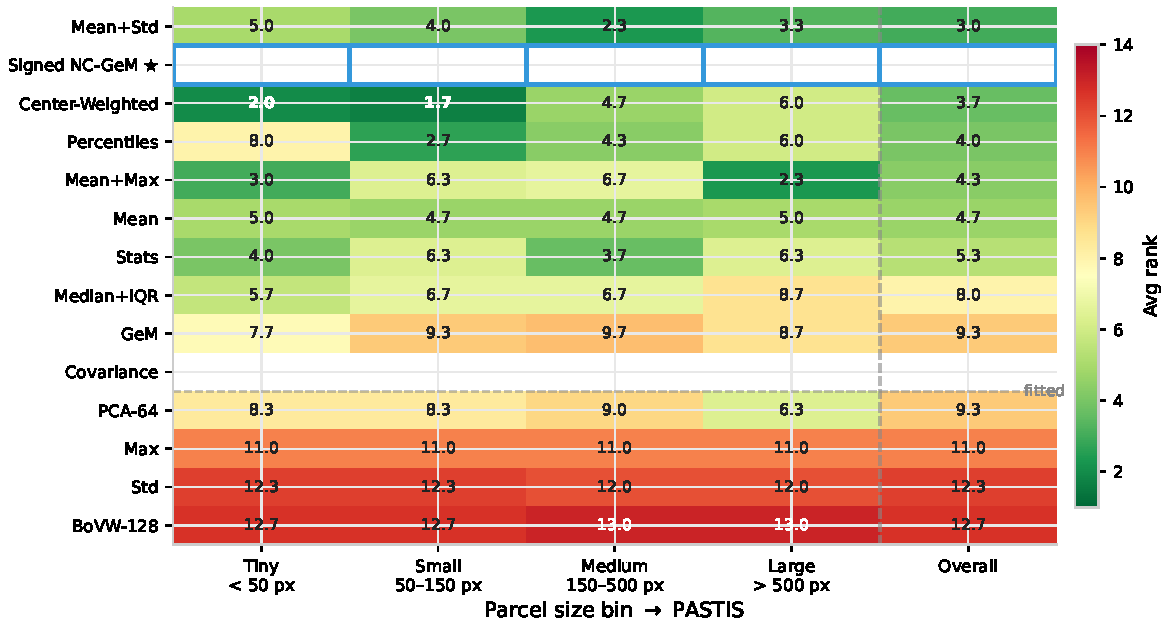
\includegraphics[width=\linewidth]{ranking_heatmap.pdf}
  \caption{\textbf{Method rankings shift as parcel size grows.} Each cell shows the average rank across AEF, OlmoEarth, and Tessera within each parcel-size bin---darker blue is a better rank (1=best). Center-weighted mean and mean+max dominate the tiny bin; mean+std rises as parcels grow; covariance moves from near-bottom (tiny/small) to mid-pack (large) but never leads at the parcel scale, since $N/D$ remains modest. Mean+std ($\bigstar$, highlighted in orange) is the only training-free method that stays in the top~3 for the small, medium, and large bins. The dashed vertical line separates per-bin results from the overall ranking.}
  \label{fig:ranking_heatmap}
\end{figure}

\section{Discussion}

\begin{table}[!t]
  \centering
  \footnotesize
  \setlength{\tabcolsep}{4pt}
  \caption{Practitioner cheat-sheet: pick a pooling operator from $N$ (pixels per region) and $D$ (embedding dimension). Apply at inference time, no training.}\label{tab:cheatsheet}
  \begin{tabular}{@{}p{0.30\linewidth}p{0.36\linewidth}p{0.22\linewidth}@{}}
    \toprule
    Regime & Recommended & Fallback \\
    \midrule
    $N \gg D$ (fixed chips, $\gtrsim$\,1k px) & \textit{stats} (or \textit{covariance}) & \textit{mean+std} \\
    $N \approx D$ or variable-size regions & \textit{mean+std} & \textit{center-weighted} \\
    Tiny ($N < D$) & \textit{center-weighted} or \textit{mean+max} & \textit{mean+std} \\
    \bottomrule
  \end{tabular}
\end{table}

\textbf{Recommendation.} Table~\ref{tab:cheatsheet} gives an empirical decision rule indexed by $N/D$: $N/D$ formally predicts when second-order pooling is viable, and the small/large region rows are empirical defaults supported by our two benchmarks. When $N \gg D$ (large fixed-size patches, \eg\ $64{\times}64$ at 10\,m), use \textit{stats} or \textit{covariance} for peak accuracy; \textit{stats} is more robust to distribution shift. When $N \approx D$ or regions are variable-size (parcels, fields, buildings), use \textit{mean+std}: it wins the PASTIS linear-probe average (56.4\% F1) and is the only training-free method that stays in the top-3 across the small, medium, and large parcel-size bins. For predominantly tiny regions ($N{<}D$), \textit{center-weighted mean} dominates. \textit{Mean} remains a useful lower bound. Accuracy and robustness move together here: \textit{stats} and \textit{mean+std} are simultaneously more accurate and more robust than \textit{mean}, with no observed accuracy--robustness tradeoff.

\textbf{Why distributional statistics help.} Mean pooling collapses each region to its average vector, discarding intra-region heterogeneity. A residential neighborhood and an industrial zone may share a mean embedding while differing in variance: the mean erases that distinction; \textit{stats} and \textit{mean+std} preserve it. This signal is reliable only when $N$ is large enough to estimate higher moments---which is precisely what $N/D$ measures.

\textbf{Practical applications.} The decision rule maps directly onto GIS zonal-statistics workflows~\cite{cressie2015statistics,eo4geoobia}, where raster values are aggregated over vector polygons (agricultural fields, building footprints, administrative units, ecological zones). As GFM embedding products become available at continental scale~\cite{fang2026earthembeddingsproductstaxonomy}, practitioners running polygon-level inference---crop monitoring~\cite{kerner2025ftw}, habitat classification, urban mapping---can apply Table~\ref{tab:cheatsheet} at inference time with no additional training.

\textbf{Related work.} GFM embedding products have proliferated~\cite{jakubik2023prithvi,cong2022satmae,bastani2023satlaspretrain,brown2025alphaearth,herzog2025olmoearth,feng2025tesseratemporalembeddingssurface}, but post-hoc pooling for these embeddings is largely unstudied; the closest prior comparisons are in image retrieval (GeM~\cite{radenovic2018gem}, VLAD~\cite{jegou2010vlad}, NetVLAD~\cite{arandjelovic2016netvlad}, Fisher vectors~\cite{perronnin2010improving}), bilinear/covariance pooling~\cite{lin2015bilinear}, and aggregation in temporal audio~\cite{miech2017learnable}. Our setting differs in that $N$ varies by three orders of magnitude across regions, which is what makes the $N/D$ ratio actionable.

\textbf{Limitations.} We evaluate on EuroSAT (10 classes) and PASTIS (18 crop classes), both Sentinel-2 at 10\,m, with three embedding sources; broader coverage (\eg, BigEarthNet~\cite{sumbul2019bigearthnet}, fMoW~\cite{christie2018functional}, multi-label or dense-prediction settings) would strengthen conclusions. OlmoEarth is evaluated with $T{=}12$ subsampled time steps; AEF and Tessera use the encoders' default annual representation. The temporal aggregation strategy per encoder is fixed rather than ablated. We study only patch- and parcel-level labels, not semantic segmentation. We focus on training-free pooling; learned aggregation~\cite{touvron2022augmenting} may improve further but requires encoder access.

\section{Conclusion}

The pixel-to-dimension ratio $N/D$ is a principled, single-number criterion for whether second-order pooling of GFM embeddings is viable, anchoring an otherwise empirical operator choice. We give a one-step recommendation in Table~\ref{tab:cheatsheet} that practitioners can apply at inference time, and release \emph{EuroSAT-Embed}, \emph{PASTIS-Embed}, and benchmark code to reproduce every result.

\bibliographystyle{IEEEtran}
\bibliography{refs}

\end{document}
